\documentclass[12pt]{article}
 
\usepackage{amssymb,amsfonts,amsmath}
\usepackage{bm}
\usepackage{dsfont}
\usepackage{color,soul}
\usepackage{graphicx}
\usepackage{caption}

%%%>

\usepackage{float}
\usepackage{hyperref}

\usepackage{tikz}
\usetikzlibrary{backgrounds,fit,decorations.pathreplacing,calc}

\newcommand{\ket}[1]{\ensuremath{\left| #1 \right \rangle}}
\newcommand{\bra}[1]{\ensuremath{\left \langle #1 \right |}}
\newcommand{\braket}[2]{\ensuremath{\left\langle #1\left|#2 \right.\right\rangle}}
\def\ketbra#1#2{{\vert#1\rangle\!\langle#2\vert}}

\newcommand{\1}[1]{\mathds{1}\left[#1\right]}
\DeclareMathOperator{\Tr}{Tr}

\newtheorem{remark}{Remark}
\newtheorem{definition}{Definition}
\newtheorem{theorem}{Theorem}
\newtheorem{lemma}{Lemma}
\newtheorem{example}{Example}

\usepackage{bbm}

\newcommand{\eye}{\mathds{1}} % vector space identity op
%\usepackage[dvipsnames]{xcolor}
\usepackage[colorinlistoftodos,textsize=small,backgroundcolor=BlueGreen,linecolor=Blue]{todonotes}


\title{Deutsch-Jozsa Circuits using the $Z^n$-gate as Oracle (Tikz).}
\date{\today}

\author{}

%\homepage{DeepQuantum.AI}

\begin{document}
\maketitle

%\subsection{}

\section*{1 qubit}


\begin{center}
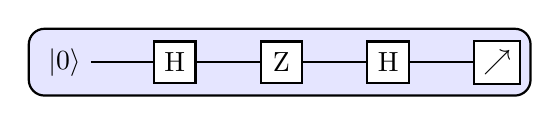
\begin{tikzpicture}[thick]
    % `operator' will only be used by Hadamard (H) gates here.
    % `phase' is used for controlled phase gates (dots).
    % `surround' is used for the background box.
    \tikzstyle{operator} = [draw,fill=white,minimum size=1.5em] 
    \tikzstyle{phase} = [draw,fill,shape=circle,minimum size=5pt,inner sep=0pt]
    \tikzstyle{surround} = [fill=blue!10,thick,draw=black,rounded corners=2mm]
    %
    \matrix[row sep=0.4cm, column sep=0.8cm] (circuit) {
    % First row.
    \node (q1) {\ket{0}}; &
    \node[operator] (X11) {H}; &
    \node[operator] (X12) {Z}; &
    \node[operator] (X13) {H}; &
    \node[operator] (X14) {$\nearrow$};
    \coordinate (end1); \\
    };
    % Draw bracket on right with resultant state.
%    \draw[decorate,decoration={brace},thick]
   %     ($(circuit.north east)-(0cm,0.3cm)$)
 %       to node[midway,right] (bracket) {}
  %      ($(circuit.south east)+(0cm,0.3cm)$);
    \begin{pgfonlayer}{background}
        % Draw background box.
        \node[surround] (background) [fit = (q1)  (X14)] {};
        % Draw lines.
        \draw[thick] (q1) -- (end1)   ;
    \end{pgfonlayer}
    %
    \end{tikzpicture}
\end{center}


\section*{2 qubits}

\begin{center}
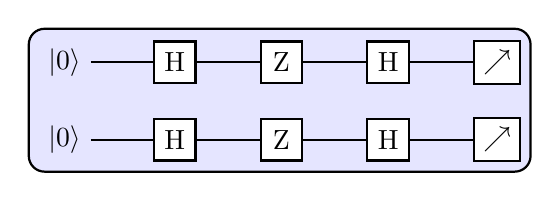
\begin{tikzpicture}[thick]
    % `operator' will only be used by Hadamard (H) gates here.
    % `phase' is used for controlled phase gates (dots).
    % `surround' is used for the background box.
    \tikzstyle{operator} = [draw,fill=white,minimum size=1.5em] 
    \tikzstyle{phase} = [draw,fill,shape=circle,minimum size=5pt,inner sep=0pt]
    \tikzstyle{surround} = [fill=blue!10,thick,draw=black,rounded corners=2mm]
    %
    \matrix[row sep=0.4cm, column sep=0.8cm] (circuit) {
    % First row.
    \node (q1) {\ket{0}}; &
    \node[operator] (X11) {H}; &
    \node[operator] (X12) {Z}; &
    \node[operator] (X13) {H}; &
    \node[operator] (X14) {$\nearrow$};
    \coordinate (end1); \\
    % Second row.
    \node (q2) {\ket{0}}; &
    \node[operator] (X21) {H}; &
    \node[operator] (X22) {Z}; &
    \node[operator] (X23) {H}; &
    \node[operator] (X24) {$\nearrow$};

    \coordinate (end2);\\
    };
    % Draw bracket on right with resultant state.
%    \draw[decorate,decoration={brace},thick]
   %     ($(circuit.north east)-(0cm,0.3cm)$)
 %       to node[midway,right] (bracket) {}
  %      ($(circuit.south east)+(0cm,0.3cm)$);
    \begin{pgfonlayer}{background}
        % Draw background box.
        \node[surround] (background) [fit = (q1)  (X24)] {};
        % Draw lines.
        \draw[thick] (q1) -- (end1)  (q2) -- (end2) ;
    \end{pgfonlayer}
    %
    \end{tikzpicture}
\end{center}


\section*{3 qubits}


\begin{center}
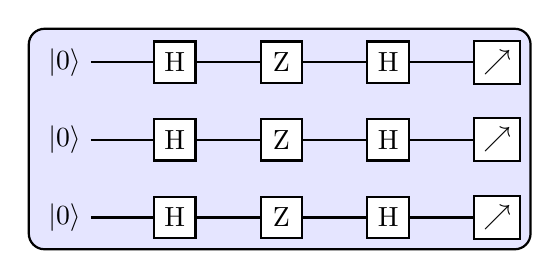
\begin{tikzpicture}[thick]
    % `operator' will only be used by Hadamard (H) gates here.
    % `phase' is used for controlled phase gates (dots).
    % `surround' is used for the background box.
    \tikzstyle{operator} = [draw,fill=white,minimum size=1.5em] 
    \tikzstyle{phase} = [draw,fill,shape=circle,minimum size=5pt,inner sep=0pt]
    \tikzstyle{surround} = [fill=blue!10,thick,draw=black,rounded corners=2mm]
    %
    \matrix[row sep=0.4cm, column sep=0.8cm] (circuit) {
    % First row.
    \node (q1) {\ket{0}}; &
    \node[operator] (X11) {H}; &
    \node[operator] (X12) {Z}; &
    \node[operator] (X13) {H}; &
    \node[operator] (X14) {$\nearrow$};
    \coordinate (end1); \\
    % Second row.
    \node (q2) {\ket{0}}; &
    \node[operator] (X21) {H}; &
    \node[operator] (X22) {Z}; &
    \node[operator] (X23) {H}; &
    \node[operator] (X24) {$\nearrow$};

    \coordinate (end2);\\
    % Third row.
    \node (q3) {\ket{0}}; &
    \node[operator] (X31) {H}; &
    \node[operator] (X32) {Z}; &
    \node[operator] (X33) {H}; &
    \node[operator] (X34) {$\nearrow$};
 
    \coordinate (end3); \\
    };
    % Draw bracket on right with resultant state.
%    \draw[decorate,decoration={brace},thick]
   %     ($(circuit.north east)-(0cm,0.3cm)$)
 %       to node[midway,right] (bracket) {}
  %      ($(circuit.south east)+(0cm,0.3cm)$);
    \begin{pgfonlayer}{background}
        % Draw background box.
        \node[surround] (background) [fit = (q1)  (X34)] {};
        % Draw lines.
        \draw[thick] (q1) -- (end1)  (q2) -- (end2) (q3) -- (end3);
    \end{pgfonlayer}
    %
    \end{tikzpicture}
\end{center}

\section*{4 qubits}

\begin{center}
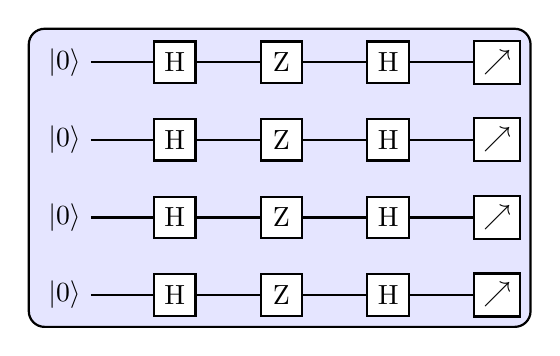
\begin{tikzpicture}[thick]
    % `operator' will only be used by Hadamard (H) gates here.
    % `phase' is used for controlled phase gates (dots).
    % `surround' is used for the background box.
    \tikzstyle{operator} = [draw,fill=white,minimum size=1.5em] 
    \tikzstyle{phase} = [draw,fill,shape=circle,minimum size=5pt,inner sep=0pt]
    \tikzstyle{surround} = [fill=blue!10,thick,draw=black,rounded corners=2mm]
    %
    \matrix[row sep=0.4cm, column sep=0.8cm] (circuit) {
    % First row.
    \node (q1) {\ket{0}}; &
    \node[operator] (X11) {H}; &
    \node[operator] (X12) {Z}; &
    \node[operator] (X13) {H}; &
    \node[operator] (X14) {$\nearrow$};
    \coordinate (end1); \\
    % Second row.
    \node (q2) {\ket{0}}; &
    \node[operator] (X21) {H}; &
    \node[operator] (X22) {Z}; &
    \node[operator] (X23) {H}; &
    \node[operator] (X24) {$\nearrow$};

    \coordinate (end2);\\
    % Third row.
    \node (q3) {\ket{0}}; &
    \node[operator] (X31) {H}; &
    \node[operator] (X32) {Z}; &
    \node[operator] (X33) {H}; &
    \node[operator] (X34) {$\nearrow$};
 
    \coordinate (end3); \\
    % Fourth row.
    \node (q4) {\ket{0}}; &
    \node[operator] (X41) {H}; &
    \node[operator] (X42) {Z}; &
    \node[operator] (X43) {H}; &
    \node[operator] (X44) {$\nearrow$};
    \coordinate (end4); \\
    };
    % Draw bracket on right with resultant state.
%    \draw[decorate,decoration={brace},thick]
   %     ($(circuit.north east)-(0cm,0.3cm)$)
 %       to node[midway,right] (bracket) {}
  %      ($(circuit.south east)+(0cm,0.3cm)$);
    \begin{pgfonlayer}{background}
        % Draw background box.
        \node[surround] (background) [fit = (q1)  (X44)] {};
        % Draw lines.
        \draw[thick] (q1) -- (end1)  (q2) -- (end2) (q3) -- (end3) (q4) -- (end4);
    \end{pgfonlayer}
    %
    \end{tikzpicture}
\end{center}

\section*{5 qubits}

\begin{center}
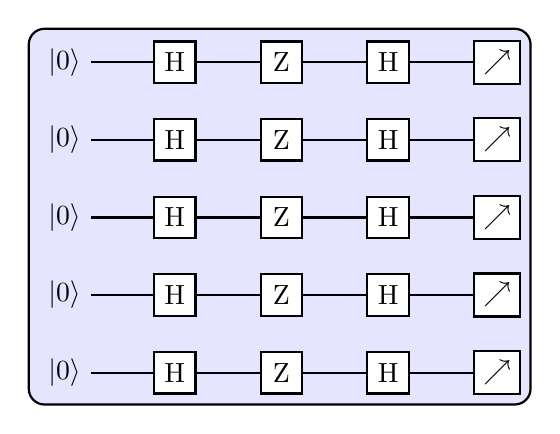
\begin{tikzpicture}[thick]
    % `operator' will only be used by Hadamard (H) gates here.
    % `phase' is used for controlled phase gates (dots).
    % `surround' is used for the background box.
    \tikzstyle{operator} = [draw,fill=white,minimum size=1.5em] 
    \tikzstyle{phase} = [draw,fill,shape=circle,minimum size=5pt,inner sep=0pt]
    \tikzstyle{surround} = [fill=blue!10,thick,draw=black,rounded corners=2mm]
    %
    \matrix[row sep=0.4cm, column sep=0.8cm] (circuit) {
    % First row.
    \node (q1) {\ket{0}}; &
    \node[operator] (X11) {H}; &
    \node[operator] (X12) {Z}; &
    \node[operator] (X13) {H}; &
    \node[operator] (X14) {$\nearrow$};
    \coordinate (end1); \\
    % Second row.
    \node (q2) {\ket{0}}; &
    \node[operator] (X21) {H}; &
    \node[operator] (X22) {Z}; &
    \node[operator] (X23) {H}; &
    \node[operator] (X24) {$\nearrow$};

    \coordinate (end2);\\
    % Third row.
    \node (q3) {\ket{0}}; &
    \node[operator] (X31) {H}; &
    \node[operator] (X32) {Z}; &
    \node[operator] (X33) {H}; &
    \node[operator] (X34) {$\nearrow$};
 
    \coordinate (end3); \\
    % Fourth row.
    \node (q4) {\ket{0}}; &
    \node[operator] (X41) {H}; &
    \node[operator] (X42) {Z}; &
    \node[operator] (X43) {H}; &
    \node[operator] (X44) {$\nearrow$};
    \coordinate (end4); \\
    % Fifth row.
    \node (q5) {\ket{0}}; & 
    \node[operator] (X51) {H}; &
    \node[operator] (X52) {Z}; &
    \node[operator] (X53) {H}; &
    \node[operator] (X54) {$\nearrow$};
    \coordinate (end5); \\
    };
    % Draw bracket on right with resultant state.
%    \draw[decorate,decoration={brace},thick]
   %     ($(circuit.north east)-(0cm,0.3cm)$)
 %       to node[midway,right] (bracket) {}
  %      ($(circuit.south east)+(0cm,0.3cm)$);
    \begin{pgfonlayer}{background}
        % Draw background box.
        \node[surround] (background) [fit = (q1)  (X54)] {};
        % Draw lines.
        \draw[thick] (q1) -- (end1)  (q2) -- (end2) (q3) -- (end3) (q4) -- (end4) (q5) -- (end5)  ;
    \end{pgfonlayer}
    %
    \end{tikzpicture}
\end{center}


\section*{6 qubits}


\begin{center}
    
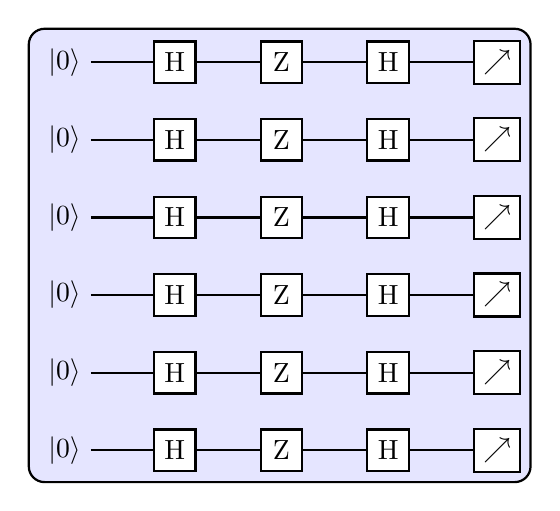
\begin{tikzpicture}[thick]
    % `operator' will only be used by Hadamard (H) gates here.
    % `phase' is used for controlled phase gates (dots).
    % `surround' is used for the background box.
    \tikzstyle{operator} = [draw,fill=white,minimum size=1.5em] 
    \tikzstyle{phase} = [draw,fill,shape=circle,minimum size=5pt,inner sep=0pt]
    \tikzstyle{surround} = [fill=blue!10,thick,draw=black,rounded corners=2mm]
    %
    \matrix[row sep=0.4cm, column sep=0.8cm] (circuit) {
    % First row.
    \node (q1) {\ket{0}}; &
    \node[operator] (X11) {H}; &
    \node[operator] (X12) {Z}; &
    \node[operator] (X13) {H}; &
    \node[operator] (X14) {$\nearrow$};
    \coordinate (end1); \\
    % Second row.
    \node (q2) {\ket{0}}; &
    \node[operator] (X21) {H}; &
    \node[operator] (X22) {Z}; &
    \node[operator] (X23) {H}; &
    \node[operator] (X24) {$\nearrow$};

    \coordinate (end2);\\
    % Third row.
    \node (q3) {\ket{0}}; &
    \node[operator] (X31) {H}; &
    \node[operator] (X32) {Z}; &
    \node[operator] (X33) {H}; &
    \node[operator] (X34) {$\nearrow$};
 
    \coordinate (end3); \\
    % Fourth row.
    \node (q4) {\ket{0}}; &
    \node[operator] (X41) {H}; &
    \node[operator] (X42) {Z}; &
    \node[operator] (X43) {H}; &
    \node[operator] (X44) {$\nearrow$};
    \coordinate (end4); \\
    % Fifth row.
    \node (q5) {\ket{0}}; & 
    \node[operator] (X51) {H}; &
    \node[operator] (X52) {Z}; &
    \node[operator] (X53) {H}; &
    \node[operator] (X54) {$\nearrow$};
    \coordinate (end5); \\
    % Sixth row.
    \node (q6) {\ket{0}}; & 
     \node[operator] (x61) {H}; &
    \node[operator] (X62) {Z}; &
    \node[operator] (X63) {H}; &
    \node[operator] (X64) {$\nearrow$};
    \coordinate (end6); \\
    };
    % Draw bracket on right with resultant state.
%    \draw[decorate,decoration={brace},thick]
   %     ($(circuit.north east)-(0cm,0.3cm)$)
 %       to node[midway,right] (bracket) {}
  %      ($(circuit.south east)+(0cm,0.3cm)$);
    \begin{pgfonlayer}{background}
        % Draw background box.
        \node[surround] (background) [fit = (q1)  (X64)] {};
        % Draw lines.
        \draw[thick] (q1) -- (end1)  (q2) -- (end2) (q3) -- (end3) (q4) -- (end4) (q5) -- (end5) (q6) -- (end6)    ;
    \end{pgfonlayer}
    %
    \end{tikzpicture}
\end{center}

\section*{7 qubits}

\begin{center}
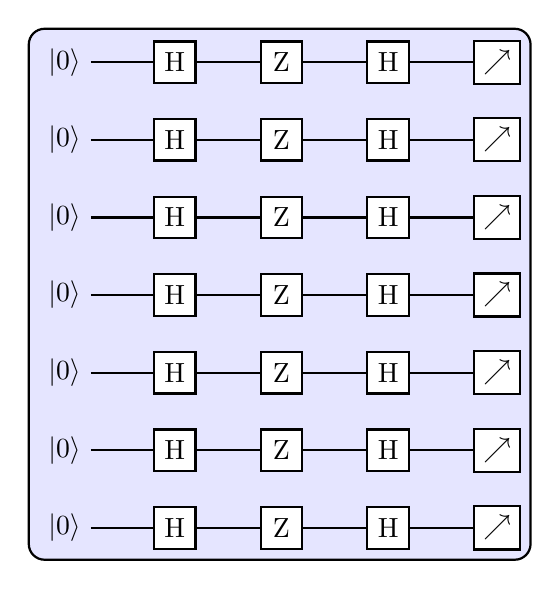
\begin{tikzpicture}[thick]
    % `operator' will only be used by Hadamard (H) gates here.
    % `phase' is used for controlled phase gates (dots).
    % `surround' is used for the background box.
    \tikzstyle{operator} = [draw,fill=white,minimum size=1.5em] 
    \tikzstyle{phase} = [draw,fill,shape=circle,minimum size=5pt,inner sep=0pt]
    \tikzstyle{surround} = [fill=blue!10,thick,draw=black,rounded corners=2mm]
    %
    \matrix[row sep=0.4cm, column sep=0.8cm] (circuit) {
    % First row.
    \node (q1) {\ket{0}}; &
    \node[operator] (X11) {H}; &
    \node[operator] (X12) {Z}; &
    \node[operator] (X13) {H}; &
    \node[operator] (X14) {$\nearrow$};
    \coordinate (end1); \\
    % Second row.
    \node (q2) {\ket{0}}; &
    \node[operator] (X21) {H}; &
    \node[operator] (X22) {Z}; &
    \node[operator] (X23) {H}; &
    \node[operator] (X24) {$\nearrow$};

    \coordinate (end2);\\
    % Third row.
    \node (q3) {\ket{0}}; &
    \node[operator] (X31) {H}; &
    \node[operator] (X32) {Z}; &
    \node[operator] (X33) {H}; &
    \node[operator] (X34) {$\nearrow$};
 
    \coordinate (end3); \\
    % Fourth row.
    \node (q4) {\ket{0}}; &
    \node[operator] (X41) {H}; &
    \node[operator] (X42) {Z}; &
    \node[operator] (X43) {H}; &
    \node[operator] (X44) {$\nearrow$};
    \coordinate (end4); \\
    % Fifth row.
    \node (q5) {\ket{0}}; & 
    \node[operator] (X51) {H}; &
    \node[operator] (X52) {Z}; &
    \node[operator] (X53) {H}; &
    \node[operator] (X54) {$\nearrow$};
    \coordinate (end5); \\
    % Sixth row.
    \node (q6) {\ket{0}}; & 
    \node[operator] (x61) {H}; &
    \node[operator] (X62) {Z}; &
    \node[operator] (X63) {H}; &
    \node[operator] (X64) {$\nearrow$};
    \coordinate (end6); \\
    
    
    \node (q7) {\ket{0}}; &
    \node[operator] (x61) {H}; &
    \node[operator] (X72) {Z}; &
    \node[operator] (X73) {H}; &
    \node[operator] (X74) {$\nearrow$};
    \coordinate (end7); \\
    };
    % Draw bracket on right with resultant state.
%    \draw[decorate,decoration={brace},thick]
   %     ($(circuit.north east)-(0cm,0.3cm)$)
 %       to node[midway,right] (bracket) {}
  %      ($(circuit.south east)+(0cm,0.3cm)$);
    \begin{pgfonlayer}{background}
        % Draw background box.
        \node[surround] (background) [fit = (q1)  (X74)] {};
        % Draw lines.
        \draw[thick] (q1) -- (end1)  (q2) -- (end2) (q3) -- (end3) (q4) -- (end4) (q5) -- (end5) (q6) -- (end6)   (q7) -- (end7) ;
    \end{pgfonlayer}
    %
    \end{tikzpicture}
\end{center}


\section*{8 qubits}


\begin{center}
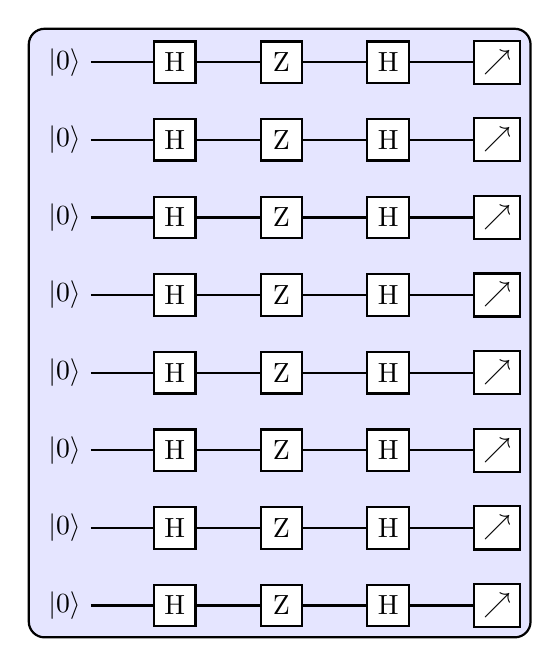
\begin{tikzpicture}[thick]
    % `operator' will only be used by Hadamard (H) gates here.
    % `phase' is used for controlled phase gates (dots).
    % `surround' is used for the background box.
    \tikzstyle{operator} = [draw,fill=white,minimum size=1.5em] 
    \tikzstyle{phase} = [draw,fill,shape=circle,minimum size=5pt,inner sep=0pt]
    \tikzstyle{surround} = [fill=blue!10,thick,draw=black,rounded corners=2mm]
    %
    \matrix[row sep=0.4cm, column sep=0.8cm] (circuit) {
    % First row.
    \node (q1) {\ket{0}}; &
    \node[operator] (X11) {H}; &
    \node[operator] (X12) {Z}; &
    \node[operator] (X13) {H}; &
    \node[operator] (X14) {$\nearrow$};
    \coordinate (end1); \\
    % Second row.
    \node (q2) {\ket{0}}; &
    \node[operator] (X21) {H}; &
    \node[operator] (X22) {Z}; &
    \node[operator] (X23) {H}; &
    \node[operator] (X24) {$\nearrow$};

    \coordinate (end2);\\
    % Third row.
    \node (q3) {\ket{0}}; &
    \node[operator] (X31) {H}; &
    \node[operator] (X32) {Z}; &
    \node[operator] (X33) {H}; &
    \node[operator] (X34) {$\nearrow$};
 
    \coordinate (end3); \\
    % Fourth row.
    \node (q4) {\ket{0}}; &
    \node[operator] (X41) {H}; &
    \node[operator] (X42) {Z}; &
    \node[operator] (X43) {H}; &
    \node[operator] (X44) {$\nearrow$};
    \coordinate (end4); \\
    % Fifth row.
    \node (q5) {\ket{0}}; & 
    \node[operator] (X51) {H}; &
    \node[operator] (X52) {Z}; &
    \node[operator] (X53) {H}; &
    \node[operator] (X54) {$\nearrow$};
    \coordinate (end5); \\
    % Sixth row.
    \node (q6) {\ket{0}}; & 
    \node[operator] (x61) {H}; &
    \node[operator] (X62) {Z}; &
    \node[operator] (X63) {H}; &
    \node[operator] (X64) {$\nearrow$};
    \coordinate (end6); \\
    
    
    \node (q7) {\ket{0}}; &
    \node[operator] (x61) {H}; &
    \node[operator] (X72) {Z}; &
    \node[operator] (X73) {H}; &
    \node[operator] (X74) {$\nearrow$};
    \coordinate (end7); \\
    
    \node (q8) {\ket{0}}; &
    \node[operator] (x81) {H}; &
    \node[operator] (X82) {Z}; &
    \node[operator] (X83) {H}; &
    \node[operator] (X84) {$\nearrow$};
    \coordinate (end8); \\
    };
    % Draw bracket on right with resultant state.
%    \draw[decorate,decoration={brace},thick]
   %     ($(circuit.north east)-(0cm,0.3cm)$)
 %       to node[midway,right] (bracket) {}
  %      ($(circuit.south east)+(0cm,0.3cm)$);
    \begin{pgfonlayer}{background}
        % Draw background box.
        \node[surround] (background) [fit = (q1)  (X84)] {};
        % Draw lines.
        \draw[thick] (q1) -- (end1)  (q2) -- (end2) (q3) -- (end3) (q4) -- (end4) (q5) -- (end5) (q6) -- (end6)   (q7) -- (end7) (q8) -- (end8);
    \end{pgfonlayer}
    %
    \end{tikzpicture}
\end{center}

\section*{9 qubits}

\begin{center}
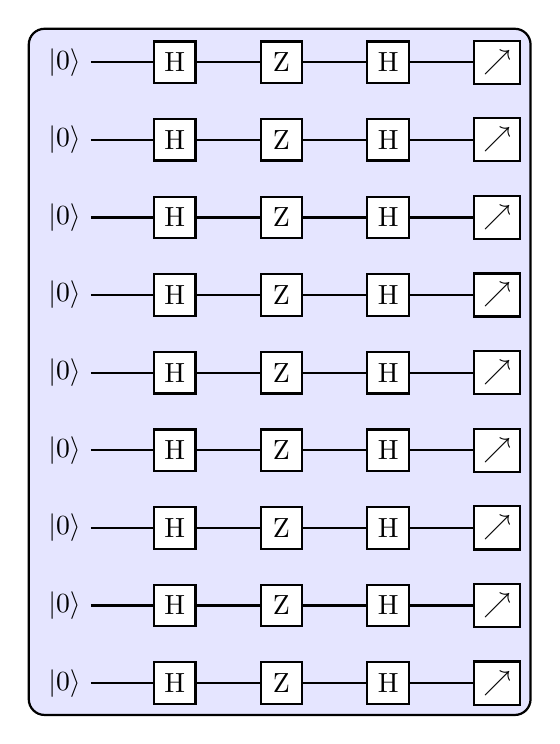
\begin{tikzpicture}[thick]
    % `operator' will only be used by Hadamard (H) gates here.
    % `phase' is used for controlled phase gates (dots).
    % `surround' is used for the background box.
    \tikzstyle{operator} = [draw,fill=white,minimum size=1.5em] 
    \tikzstyle{phase} = [draw,fill,shape=circle,minimum size=5pt,inner sep=0pt]
    \tikzstyle{surround} = [fill=blue!10,thick,draw=black,rounded corners=2mm]
    %
    \matrix[row sep=0.4cm, column sep=0.8cm] (circuit) {
    % First row.
    \node (q1) {\ket{0}}; &
    \node[operator] (X11) {H}; &
    \node[operator] (X12) {Z}; &
    \node[operator] (X13) {H}; &
    \node[operator] (X14) {$\nearrow$};
    \coordinate (end1); \\
    % Second row.
    \node (q2) {\ket{0}}; &
    \node[operator] (X21) {H}; &
    \node[operator] (X22) {Z}; &
    \node[operator] (X23) {H}; &
    \node[operator] (X24) {$\nearrow$};

    \coordinate (end2);\\
    % Third row.
    \node (q3) {\ket{0}}; &
    \node[operator] (X31) {H}; &
    \node[operator] (X32) {Z}; &
    \node[operator] (X33) {H}; &
    \node[operator] (X34) {$\nearrow$};
 
    \coordinate (end3); \\
    % Fourth row.
    \node (q4) {\ket{0}}; &
    \node[operator] (X41) {H}; &
    \node[operator] (X42) {Z}; &
    \node[operator] (X43) {H}; &
    \node[operator] (X44) {$\nearrow$};
    \coordinate (end4); \\
    % Fifth row.
    \node (q5) {\ket{0}}; & 
    \node[operator] (X51) {H}; &
    \node[operator] (X52) {Z}; &
    \node[operator] (X53) {H}; &
    \node[operator] (X54) {$\nearrow$};
    \coordinate (end5); \\
    % Sixth row.
    \node (q6) {\ket{0}}; & 
    \node[operator] (x61) {H}; &
    \node[operator] (X62) {Z}; &
    \node[operator] (X63) {H}; &
    \node[operator] (X64) {$\nearrow$};
    \coordinate (end6); \\
    
    
    \node (q7) {\ket{0}}; &
    \node[operator] (x61) {H}; &
    \node[operator] (X72) {Z}; &
    \node[operator] (X73) {H}; &
    \node[operator] (X74) {$\nearrow$};
    \coordinate (end7); \\
    
    \node (q8) {\ket{0}}; &
    \node[operator] (x81) {H}; &
    \node[operator] (X82) {Z}; &
    \node[operator] (X83) {H}; &
    \node[operator] (X84) {$\nearrow$};
    \coordinate (end8); \\
    
    \node (q9) {\ket{0}}; &
    \node[operator] (x91) {H}; &
    \node[operator] (X92) {Z}; &
    \node[operator] (X93) {H}; &
    \node[operator] (X94) {$\nearrow$};
    \coordinate (end9); \\
    };
    % Draw bracket on right with resultant state.
%    \draw[decorate,decoration={brace},thick]
   %     ($(circuit.north east)-(0cm,0.3cm)$)
 %       to node[midway,right] (bracket) {}
  %      ($(circuit.south east)+(0cm,0.3cm)$);
    \begin{pgfonlayer}{background}
        % Draw background box.
        \node[surround] (background) [fit = (q1)  (X94)] {};
        % Draw lines.
        \draw[thick] (q1) -- (end1)  (q2) -- (end2) (q3) -- (end3) (q4) -- (end4) (q5) -- (end5) (q6) -- (end6)   (q7) -- (end7) (q8) -- (end8) (q9) -- (end9);
    \end{pgfonlayer}
    %
    \end{tikzpicture}
\end{center}


\section*{10 qubits}

\begin{center}
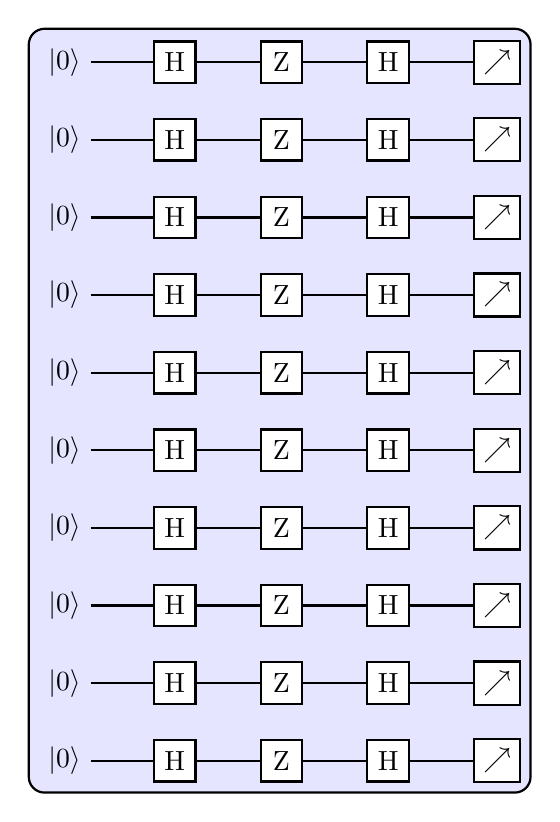
\begin{tikzpicture}[thick]
    % `operator' will only be used by Hadamard (H) gates here.
    % `phase' is used for controlled phase gates (dots).
    % `surround' is used for the background box.
    \tikzstyle{operator} = [draw,fill=white,minimum size=1.5em] 
    \tikzstyle{phase} = [draw,fill,shape=circle,minimum size=5pt,inner sep=0pt]
    \tikzstyle{surround} = [fill=blue!10,thick,draw=black,rounded corners=2mm]
    %
    \matrix[row sep=0.4cm, column sep=0.8cm] (circuit) {
    % First row.
    \node (q1) {\ket{0}}; &
    \node[operator] (X11) {H}; &
    \node[operator] (X12) {Z}; &
    \node[operator] (X13) {H}; &
    \node[operator] (X14) {$\nearrow$};
    \coordinate (end1); \\
    % Second row.
    \node (q2) {\ket{0}}; &
    \node[operator] (X21) {H}; &
    \node[operator] (X22) {Z}; &
    \node[operator] (X23) {H}; &
    \node[operator] (X24) {$\nearrow$};

    \coordinate (end2);\\
    % Third row.
    \node (q3) {\ket{0}}; &
    \node[operator] (X31) {H}; &
    \node[operator] (X32) {Z}; &
    \node[operator] (X33) {H}; &
    \node[operator] (X34) {$\nearrow$};
 
    \coordinate (end3); \\
    % Fourth row.
    \node (q4) {\ket{0}}; &
    \node[operator] (X41) {H}; &
    \node[operator] (X42) {Z}; &
    \node[operator] (X43) {H}; &
    \node[operator] (X44) {$\nearrow$};
    \coordinate (end4); \\
    % Fifth row.
    \node (q5) {\ket{0}}; & 
    \node[operator] (X51) {H}; &
    \node[operator] (X52) {Z}; &
    \node[operator] (X53) {H}; &
    \node[operator] (X54) {$\nearrow$};
    \coordinate (end5); \\
    % Sixth row.
    \node (q6) {\ket{0}}; & 
    \node[operator] (x61) {H}; &
    \node[operator] (X62) {Z}; &
    \node[operator] (X63) {H}; &
    \node[operator] (X64) {$\nearrow$};
    \coordinate (end6); \\
    
    
    \node (q7) {\ket{0}}; &
    \node[operator] (x61) {H}; &
    \node[operator] (X72) {Z}; &
    \node[operator] (X73) {H}; &
    \node[operator] (X74) {$\nearrow$};
    \coordinate (end7); \\
    
    \node (q8) {\ket{0}}; &
    \node[operator] (x81) {H}; &
    \node[operator] (X82) {Z}; &
    \node[operator] (X83) {H}; &
    \node[operator] (X84) {$\nearrow$};
    \coordinate (end8); \\
    
    \node (q9) {\ket{0}}; &
    \node[operator] (x91) {H}; &
    \node[operator] (X92) {Z}; &
    \node[operator] (X93) {H}; &
    \node[operator] (X94) {$\nearrow$};
    \coordinate (end9); \\
    
        \node (q10) {\ket{0}}; &
    \node[operator] (x101) {H}; &
    \node[operator] (X102) {Z}; &
    \node[operator] (X103) {H}; &
    \node[operator] (X104) {$\nearrow$};
    \coordinate (end10); \\
    };
    % Draw bracket on right with resultant state.
%    \draw[decorate,decoration={brace},thick]
   %     ($(circuit.north east)-(0cm,0.3cm)$)
 %       to node[midway,right] (bracket) {}
  %      ($(circuit.south east)+(0cm,0.3cm)$);
    \begin{pgfonlayer}{background}
        % Draw background box.
        \node[surround] (background) [fit = (q1)  (X94) (X104)] {};
        % Draw lines.
        \draw[thick] (q1) -- (end1)  (q2) -- (end2) (q3) -- (end3) (q4) -- (end4) (q5) -- (end5) (q6) -- (end6)   (q7) -- (end7) (q8) -- (end8) (q9) -- (end9) (q10) -- (end10);
    \end{pgfonlayer}
    %
    \end{tikzpicture}
\end{center}


\section*{11 qubits}

\begin{center}
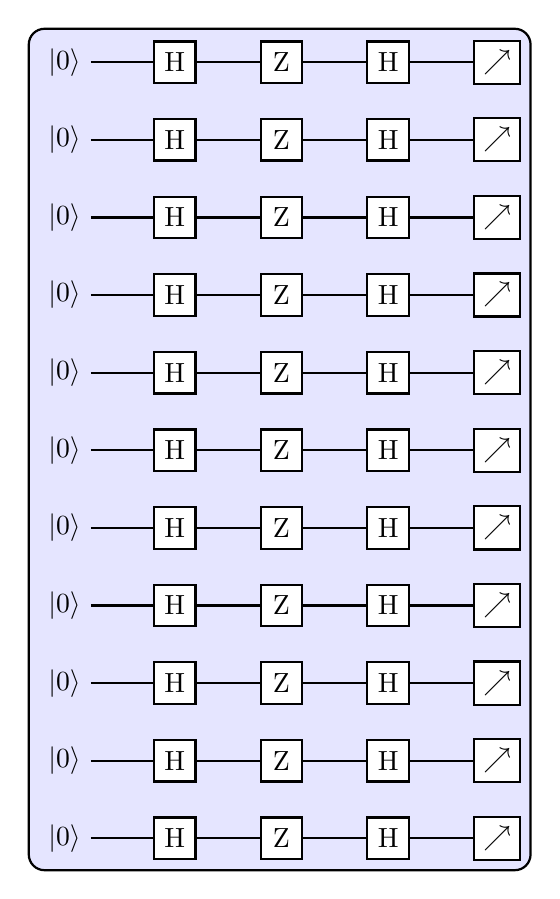
\begin{tikzpicture}[thick]
    % `operator' will only be used by Hadamard (H) gates here.
    % `phase' is used for controlled phase gates (dots).
    % `surround' is used for the background box.
    \tikzstyle{operator} = [draw,fill=white,minimum size=1.5em] 
    \tikzstyle{phase} = [draw,fill,shape=circle,minimum size=5pt,inner sep=0pt]
    \tikzstyle{surround} = [fill=blue!10,thick,draw=black,rounded corners=2mm]
    %
    \matrix[row sep=0.4cm, column sep=0.8cm] (circuit) {
    % First row.
    \node (q1) {\ket{0}}; &
    \node[operator] (X11) {H}; &
    \node[operator] (X12) {Z}; &
    \node[operator] (X13) {H}; &
    \node[operator] (X14) {$\nearrow$};
    \coordinate (end1); \\
    % Second row.
    \node (q2) {\ket{0}}; &
    \node[operator] (X21) {H}; &
    \node[operator] (X22) {Z}; &
    \node[operator] (X23) {H}; &
    \node[operator] (X24) {$\nearrow$};

    \coordinate (end2);\\
    % Third row.
    \node (q3) {\ket{0}}; &
    \node[operator] (X31) {H}; &
    \node[operator] (X32) {Z}; &
    \node[operator] (X33) {H}; &
    \node[operator] (X34) {$\nearrow$};
 
    \coordinate (end3); \\
    % Fourth row.
    \node (q4) {\ket{0}}; &
    \node[operator] (X41) {H}; &
    \node[operator] (X42) {Z}; &
    \node[operator] (X43) {H}; &
    \node[operator] (X44) {$\nearrow$};
    \coordinate (end4); \\
    % Fifth row.
    \node (q5) {\ket{0}}; & 
    \node[operator] (X51) {H}; &
    \node[operator] (X52) {Z}; &
    \node[operator] (X53) {H}; &
    \node[operator] (X54) {$\nearrow$};
    \coordinate (end5); \\
    % Sixth row.
    \node (q6) {\ket{0}}; & 
    \node[operator] (x61) {H}; &
    \node[operator] (X62) {Z}; &
    \node[operator] (X63) {H}; &
    \node[operator] (X64) {$\nearrow$};
    \coordinate (end6); \\
    
    
    \node (q7) {\ket{0}}; &
    \node[operator] (x61) {H}; &
    \node[operator] (X72) {Z}; &
    \node[operator] (X73) {H}; &
    \node[operator] (X74) {$\nearrow$};
    \coordinate (end7); \\
    
    \node (q8) {\ket{0}}; &
    \node[operator] (x81) {H}; &
    \node[operator] (X82) {Z}; &
    \node[operator] (X83) {H}; &
    \node[operator] (X84) {$\nearrow$};
    \coordinate (end8); \\
    
    \node (q9) {\ket{0}}; &
    \node[operator] (x91) {H}; &
    \node[operator] (X92) {Z}; &
    \node[operator] (X93) {H}; &
    \node[operator] (X94) {$\nearrow$};
    \coordinate (end9); \\
    
        \node (q10) {\ket{0}}; &
    \node[operator] (x101) {H}; &
    \node[operator] (X102) {Z}; &
    \node[operator] (X103) {H}; &
    \node[operator] (X104) {$\nearrow$};
    \coordinate (end10); \\
    
      \node (q11) {\ket{0}}; &
    \node[operator] (x111) {H}; &
    \node[operator] (X112) {Z}; &
    \node[operator] (X113) {H}; &
    \node[operator] (X114) {$\nearrow$};
    \coordinate (end11); \\
    };
    % Draw bracket on right with resultant state.
%    \draw[decorate,decoration={brace},thick]
   %     ($(circuit.north east)-(0cm,0.3cm)$)
 %       to node[midway,right] (bracket) {}
  %      ($(circuit.south east)+(0cm,0.3cm)$);
    \begin{pgfonlayer}{background}
        % Draw background box.
        \node[surround] (background) [fit = (q1)  (X94) (X114)] {};
        % Draw lines.
        \draw[thick] (q1) -- (end1)  (q2) -- (end2) (q3) -- (end3) (q4) -- (end4) (q5) -- (end5) (q6) -- (end6)   (q7) -- (end7) (q8) -- (end8) (q9) -- (end9) (q10) -- (end10) (q11) -- (end11);
    \end{pgfonlayer}
    %
    \end{tikzpicture}
\end{center}

\section*{12 qubits}
\begin{center}
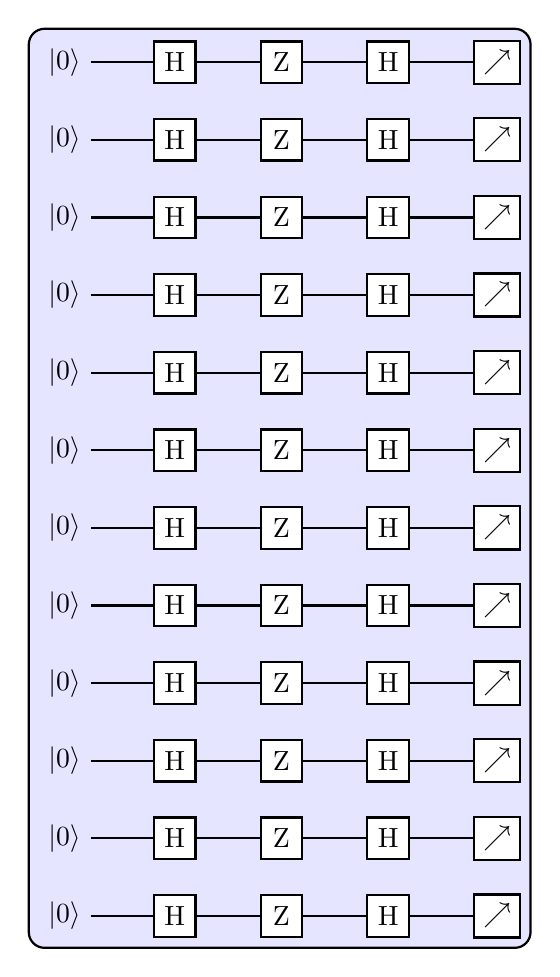
\begin{tikzpicture}[thick]
    % `operator' will only be used by Hadamard (H) gates here.
    % `phase' is used for controlled phase gates (dots).
    % `surround' is used for the background box.
    \tikzstyle{operator} = [draw,fill=white,minimum size=1.5em] 
    \tikzstyle{phase} = [draw,fill,shape=circle,minimum size=5pt,inner sep=0pt]
    \tikzstyle{surround} = [fill=blue!10,thick,draw=black,rounded corners=2mm]
    %
    \matrix[row sep=0.4cm, column sep=0.8cm] (circuit) {
    % First row.
    \node (q1) {\ket{0}}; &
    \node[operator] (X11) {H}; &
    \node[operator] (X12) {Z}; &
    \node[operator] (X13) {H}; &
    \node[operator] (X14) {$\nearrow$};
    \coordinate (end1); \\
    % Second row.
    \node (q2) {\ket{0}}; &
    \node[operator] (X21) {H}; &
    \node[operator] (X22) {Z}; &
    \node[operator] (X23) {H}; &
    \node[operator] (X24) {$\nearrow$};

    \coordinate (end2);\\
    % Third row.
    \node (q3) {\ket{0}}; &
    \node[operator] (X31) {H}; &
    \node[operator] (X32) {Z}; &
    \node[operator] (X33) {H}; &
    \node[operator] (X34) {$\nearrow$};
 
    \coordinate (end3); \\
    % Fourth row.
    \node (q4) {\ket{0}}; &
    \node[operator] (X41) {H}; &
    \node[operator] (X42) {Z}; &
    \node[operator] (X43) {H}; &
    \node[operator] (X44) {$\nearrow$};
    \coordinate (end4); \\
    % Fifth row.
    \node (q5) {\ket{0}}; & 
    \node[operator] (X51) {H}; &
    \node[operator] (X52) {Z}; &
    \node[operator] (X53) {H}; &
    \node[operator] (X54) {$\nearrow$};
    \coordinate (end5); \\
    % Sixth row.
    \node (q6) {\ket{0}}; & 
    \node[operator] (x61) {H}; &
    \node[operator] (X62) {Z}; &
    \node[operator] (X63) {H}; &
    \node[operator] (X64) {$\nearrow$};
    \coordinate (end6); \\
    
    
    \node (q7) {\ket{0}}; &
    \node[operator] (x61) {H}; &
    \node[operator] (X72) {Z}; &
    \node[operator] (X73) {H}; &
    \node[operator] (X74) {$\nearrow$};
    \coordinate (end7); \\
    
    \node (q8) {\ket{0}}; &
    \node[operator] (x81) {H}; &
    \node[operator] (X82) {Z}; &
    \node[operator] (X83) {H}; &
    \node[operator] (X84) {$\nearrow$};
    \coordinate (end8); \\
    
    \node (q9) {\ket{0}}; &
    \node[operator] (x91) {H}; &
    \node[operator] (X92) {Z}; &
    \node[operator] (X93) {H}; &
    \node[operator] (X94) {$\nearrow$};
    \coordinate (end9); \\
    
        \node (q10) {\ket{0}}; &
    \node[operator] (x101) {H}; &
    \node[operator] (X102) {Z}; &
    \node[operator] (X103) {H}; &
    \node[operator] (X104) {$\nearrow$};
    \coordinate (end10); \\
    
      \node (q11) {\ket{0}}; &
    \node[operator] (x111) {H}; &
    \node[operator] (X112) {Z}; &
    \node[operator] (X113) {H}; &
    \node[operator] (X114) {$\nearrow$};
    \coordinate (end11); \\
    
      \node (q12) {\ket{0}}; &
    \node[operator] (x121) {H}; &
    \node[operator] (X122) {Z}; &
    \node[operator] (X123) {H}; &
    \node[operator] (X124) {$\nearrow$};
    \coordinate (end12); \\
    };
    % Draw bracket on right with resultant state.
%    \draw[decorate,decoration={brace},thick]
   %     ($(circuit.north east)-(0cm,0.3cm)$)
 %       to node[midway,right] (bracket) {}
  %      ($(circuit.south east)+(0cm,0.3cm)$);
    \begin{pgfonlayer}{background}
        % Draw background box.
        \node[surround] (background) [fit = (q1)  (X94) (X124)] {};
        % Draw lines.
        \draw[thick] (q1) -- (end1)  (q2) -- (end2) (q3) -- (end3) (q4) -- (end4) (q5) -- (end5) (q6) -- (end6)   (q7) -- (end7) (q8) -- (end8) (q9) -- (end9) (q10) -- (end10) (q11) -- (end11) (q12) -- (end12);
    \end{pgfonlayer}
    %
    \end{tikzpicture}
\end{center}


\section*{13 qubits}

\begin{center}
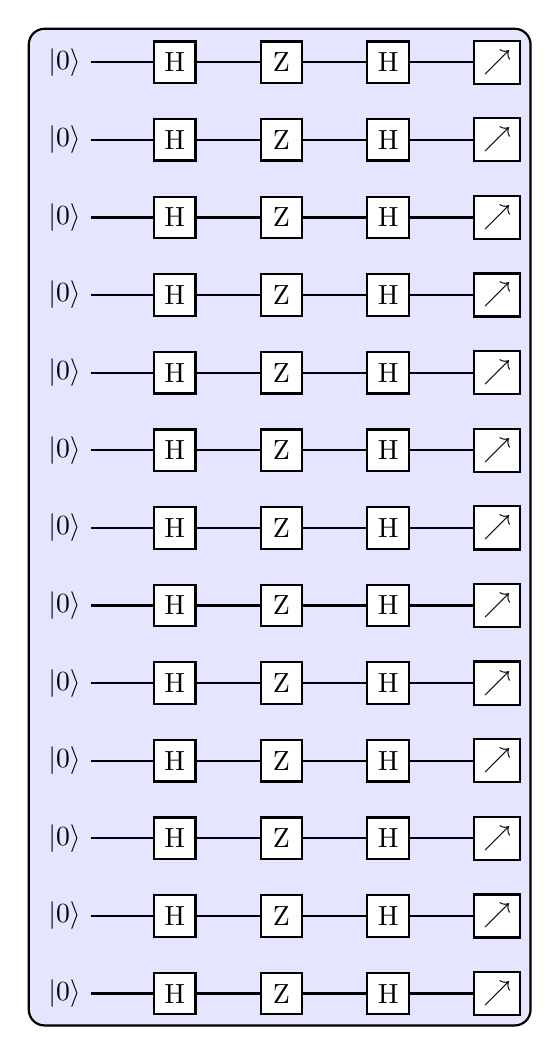
\begin{tikzpicture}[thick]
    % `operator' will only be used by Hadamard (H) gates here.
    % `phase' is used for controlled phase gates (dots).
    % `surround' is used for the background box.
    \tikzstyle{operator} = [draw,fill=white,minimum size=1.5em] 
    \tikzstyle{phase} = [draw,fill,shape=circle,minimum size=5pt,inner sep=0pt]
    \tikzstyle{surround} = [fill=blue!10,thick,draw=black,rounded corners=2mm]
    %
    \matrix[row sep=0.4cm, column sep=0.8cm] (circuit) {
    % First row.
    \node (q1) {\ket{0}}; &
    \node[operator] (X11) {H}; &
    \node[operator] (X12) {Z}; &
    \node[operator] (X13) {H}; &
    \node[operator] (X14) {$\nearrow$};
    \coordinate (end1); \\
    % Second row.
    \node (q2) {\ket{0}}; &
    \node[operator] (X21) {H}; &
    \node[operator] (X22) {Z}; &
    \node[operator] (X23) {H}; &
    \node[operator] (X24) {$\nearrow$};

    \coordinate (end2);\\
    % Third row.
    \node (q3) {\ket{0}}; &
    \node[operator] (X31) {H}; &
    \node[operator] (X32) {Z}; &
    \node[operator] (X33) {H}; &
    \node[operator] (X34) {$\nearrow$};
 
    \coordinate (end3); \\
    % Fourth row.
    \node (q4) {\ket{0}}; &
    \node[operator] (X41) {H}; &
    \node[operator] (X42) {Z}; &
    \node[operator] (X43) {H}; &
    \node[operator] (X44) {$\nearrow$};
    \coordinate (end4); \\
    % Fifth row.
    \node (q5) {\ket{0}}; & 
    \node[operator] (X51) {H}; &
    \node[operator] (X52) {Z}; &
    \node[operator] (X53) {H}; &
    \node[operator] (X54) {$\nearrow$};
    \coordinate (end5); \\
    % Sixth row.
    \node (q6) {\ket{0}}; & 
    \node[operator] (x61) {H}; &
    \node[operator] (X62) {Z}; &
    \node[operator] (X63) {H}; &
    \node[operator] (X64) {$\nearrow$};
    \coordinate (end6); \\
    
    
    \node (q7) {\ket{0}}; &
    \node[operator] (x61) {H}; &
    \node[operator] (X72) {Z}; &
    \node[operator] (X73) {H}; &
    \node[operator] (X74) {$\nearrow$};
    \coordinate (end7); \\
    
    \node (q8) {\ket{0}}; &
    \node[operator] (x81) {H}; &
    \node[operator] (X82) {Z}; &
    \node[operator] (X83) {H}; &
    \node[operator] (X84) {$\nearrow$};
    \coordinate (end8); \\
    
    \node (q9) {\ket{0}}; &
    \node[operator] (x91) {H}; &
    \node[operator] (X92) {Z}; &
    \node[operator] (X93) {H}; &
    \node[operator] (X94) {$\nearrow$};
    \coordinate (end9); \\
    
        \node (q10) {\ket{0}}; &
    \node[operator] (x101) {H}; &
    \node[operator] (X102) {Z}; &
    \node[operator] (X103) {H}; &
    \node[operator] (X104) {$\nearrow$};
    \coordinate (end10); \\
    
      \node (q11) {\ket{0}}; &
    \node[operator] (x111) {H}; &
    \node[operator] (X112) {Z}; &
    \node[operator] (X113) {H}; &
    \node[operator] (X114) {$\nearrow$};
    \coordinate (end11); \\
    
      \node (q12) {\ket{0}}; &
    \node[operator] (x121) {H}; &
    \node[operator] (X122) {Z}; &
    \node[operator] (X123) {H}; &
    \node[operator] (X124) {$\nearrow$};
    \coordinate (end12); \\
    
     \node (q13) {\ket{0}}; &
    \node[operator] (x131) {H}; &
    \node[operator] (X132) {Z}; &
    \node[operator] (X133) {H}; &
    \node[operator] (X134) {$\nearrow$};
    \coordinate (end13); \\
    };
    % Draw bracket on right with resultant state.
%    \draw[decorate,decoration={brace},thick]
   %     ($(circuit.north east)-(0cm,0.3cm)$)
 %       to node[midway,right] (bracket) {}
  %      ($(circuit.south east)+(0cm,0.3cm)$);
    \begin{pgfonlayer}{background}
        % Draw background box.
        \node[surround] (background) [fit = (q1)  (X94) (X134)] {};
        % Draw lines.
        \draw[thick] (q1) -- (end1)  (q2) -- (end2) (q3) -- (end3) (q4) -- (end4) (q5) -- (end5) (q6) -- (end6)   (q7) -- (end7) (q8) -- (end8) (q9) -- (end9) (q10) -- (end10) (q11) -- (end11) (q12) -- (end12) (q13) -- (end13);
    \end{pgfonlayer}
    %
    \end{tikzpicture}
\end{center}


\section*{14 qubits}
\begin{center}
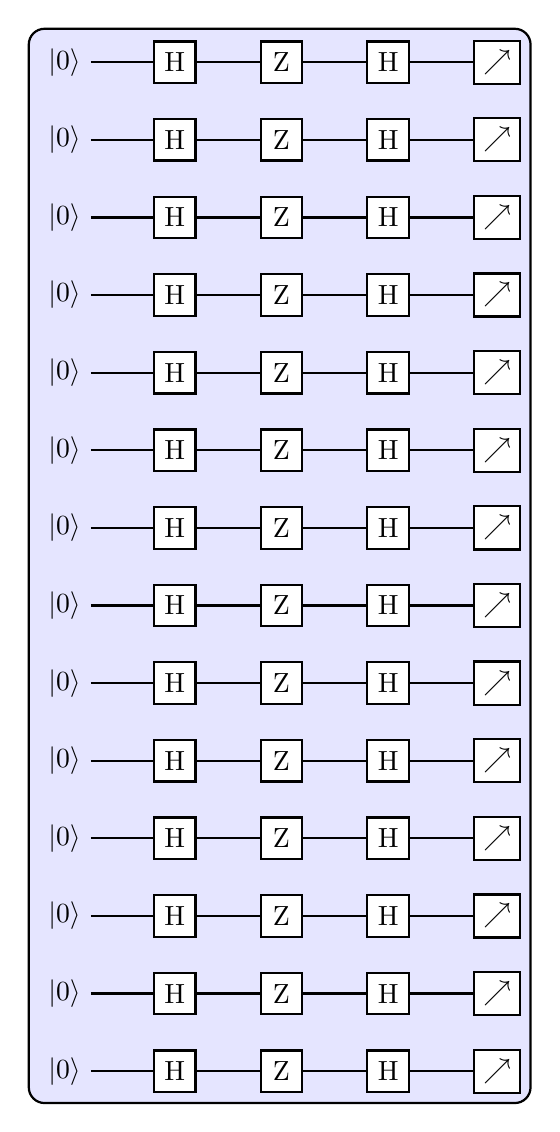
\begin{tikzpicture}[thick]
    % `operator' will only be used by Hadamard (H) gates here.
    % `phase' is used for controlled phase gates (dots).
    % `surround' is used for the background box.
    \tikzstyle{operator} = [draw,fill=white,minimum size=1.5em] 
    \tikzstyle{phase} = [draw,fill,shape=circle,minimum size=5pt,inner sep=0pt]
    \tikzstyle{surround} = [fill=blue!10,thick,draw=black,rounded corners=2mm]
    %
    \matrix[row sep=0.4cm, column sep=0.8cm] (circuit) {
    % First row.
    \node (q1) {\ket{0}}; &
    \node[operator] (X11) {H}; &
    \node[operator] (X12) {Z}; &
    \node[operator] (X13) {H}; &
    \node[operator] (X14) {$\nearrow$};
    \coordinate (end1); \\
    % Second row.
    \node (q2) {\ket{0}}; &
    \node[operator] (X21) {H}; &
    \node[operator] (X22) {Z}; &
    \node[operator] (X23) {H}; &
    \node[operator] (X24) {$\nearrow$};

    \coordinate (end2);\\
    % Third row.
    \node (q3) {\ket{0}}; &
    \node[operator] (X31) {H}; &
    \node[operator] (X32) {Z}; &
    \node[operator] (X33) {H}; &
    \node[operator] (X34) {$\nearrow$};
 
    \coordinate (end3); \\
    % Fourth row.
    \node (q4) {\ket{0}}; &
    \node[operator] (X41) {H}; &
    \node[operator] (X42) {Z}; &
    \node[operator] (X43) {H}; &
    \node[operator] (X44) {$\nearrow$};
    \coordinate (end4); \\
    % Fifth row.
    \node (q5) {\ket{0}}; & 
    \node[operator] (X51) {H}; &
    \node[operator] (X52) {Z}; &
    \node[operator] (X53) {H}; &
    \node[operator] (X54) {$\nearrow$};
    \coordinate (end5); \\
    % Sixth row.
    \node (q6) {\ket{0}}; & 
    \node[operator] (x61) {H}; &
    \node[operator] (X62) {Z}; &
    \node[operator] (X63) {H}; &
    \node[operator] (X64) {$\nearrow$};
    \coordinate (end6); \\
    
    
    \node (q7) {\ket{0}}; &
    \node[operator] (x61) {H}; &
    \node[operator] (X72) {Z}; &
    \node[operator] (X73) {H}; &
    \node[operator] (X74) {$\nearrow$};
    \coordinate (end7); \\
    
    \node (q8) {\ket{0}}; &
    \node[operator] (x81) {H}; &
    \node[operator] (X82) {Z}; &
    \node[operator] (X83) {H}; &
    \node[operator] (X84) {$\nearrow$};
    \coordinate (end8); \\
    
    \node (q9) {\ket{0}}; &
    \node[operator] (x91) {H}; &
    \node[operator] (X92) {Z}; &
    \node[operator] (X93) {H}; &
    \node[operator] (X94) {$\nearrow$};
    \coordinate (end9); \\
    
        \node (q10) {\ket{0}}; &
    \node[operator] (x101) {H}; &
    \node[operator] (X102) {Z}; &
    \node[operator] (X103) {H}; &
    \node[operator] (X104) {$\nearrow$};
    \coordinate (end10); \\
    
      \node (q11) {\ket{0}}; &
    \node[operator] (x111) {H}; &
    \node[operator] (X112) {Z}; &
    \node[operator] (X113) {H}; &
    \node[operator] (X114) {$\nearrow$};
    \coordinate (end11); \\
    
      \node (q12) {\ket{0}}; &
    \node[operator] (x121) {H}; &
    \node[operator] (X122) {Z}; &
    \node[operator] (X123) {H}; &
    \node[operator] (X124) {$\nearrow$};
    \coordinate (end12); \\
    
     \node (q13) {\ket{0}}; &
    \node[operator] (x131) {H}; &
    \node[operator] (X132) {Z}; &
    \node[operator] (X133) {H}; &
    \node[operator] (X134) {$\nearrow$};
    \coordinate (end13); \\
    
         \node (q14) {\ket{0}}; &
    \node[operator] (x141) {H}; &
    \node[operator] (X142) {Z}; &
    \node[operator] (X143) {H}; &
    \node[operator] (X144) {$\nearrow$};
    \coordinate (end14); \\
    };
    % Draw bracket on right with resultant state.
%    \draw[decorate,decoration={brace},thick]
   %     ($(circuit.north east)-(0cm,0.3cm)$)
 %       to node[midway,right] (bracket) {}
  %      ($(circuit.south east)+(0cm,0.3cm)$);
    \begin{pgfonlayer}{background}
        % Draw background box.
        \node[surround] (background) [fit = (q1)  (X94) (X144)] {};
        % Draw lines.
        \draw[thick] (q1) -- (end1)  (q2) -- (end2) (q3) -- (end3) (q4) -- (end4) (q5) -- (end5) (q6) -- (end6)   (q7) -- (end7) (q8) -- (end8) (q9) -- (end9) (q10) -- (end10) (q11) -- (end11) (q12) -- (end12) (q13) -- (end13) (q14) -- (end14);
    \end{pgfonlayer}
    %
    \end{tikzpicture}
\end{center}

\section*{15 qubits}

\begin{center}
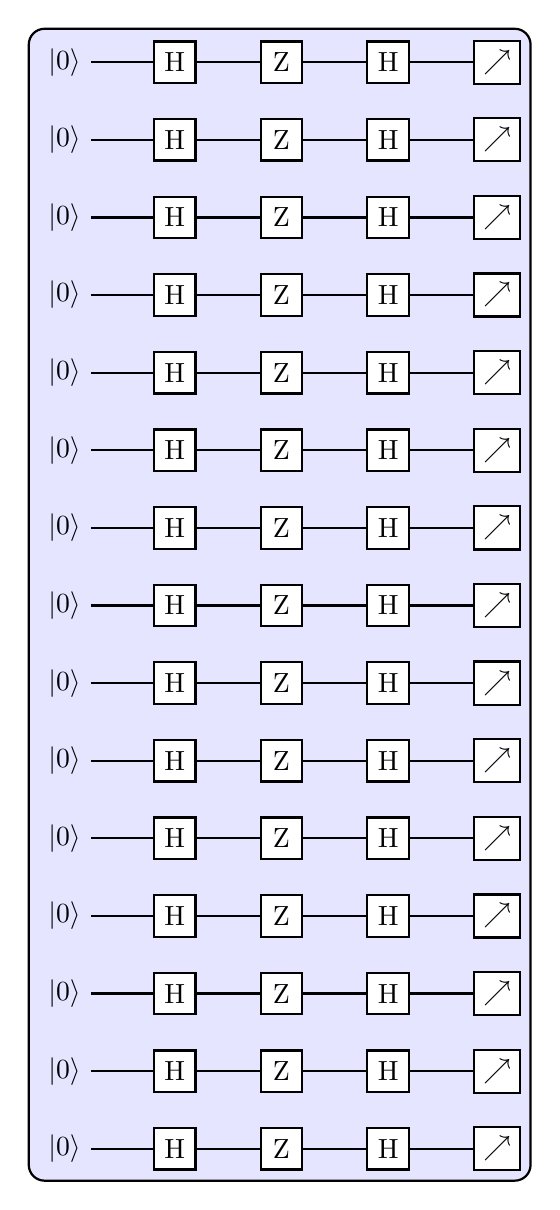
\begin{tikzpicture}[thick]
    % `operator' will only be used by Hadamard (H) gates here.
    % `phase' is used for controlled phase gates (dots).
    % `surround' is used for the background box.
    \tikzstyle{operator} = [draw,fill=white,minimum size=1.5em] 
    \tikzstyle{phase} = [draw,fill,shape=circle,minimum size=5pt,inner sep=0pt]
    \tikzstyle{surround} = [fill=blue!10,thick,draw=black,rounded corners=2mm]
    %
    \matrix[row sep=0.4cm, column sep=0.8cm] (circuit) {
    % First row.
    \node (q1) {\ket{0}}; &
    \node[operator] (X11) {H}; &
    \node[operator] (X12) {Z}; &
    \node[operator] (X13) {H}; &
    \node[operator] (X14) {$\nearrow$};
    \coordinate (end1); \\
    % Second row.
    \node (q2) {\ket{0}}; &
    \node[operator] (X21) {H}; &
    \node[operator] (X22) {Z}; &
    \node[operator] (X23) {H}; &
    \node[operator] (X24) {$\nearrow$};

    \coordinate (end2);\\
    % Third row.
    \node (q3) {\ket{0}}; &
    \node[operator] (X31) {H}; &
    \node[operator] (X32) {Z}; &
    \node[operator] (X33) {H}; &
    \node[operator] (X34) {$\nearrow$};
 
    \coordinate (end3); \\
    % Fourth row.
    \node (q4) {\ket{0}}; &
    \node[operator] (X41) {H}; &
    \node[operator] (X42) {Z}; &
    \node[operator] (X43) {H}; &
    \node[operator] (X44) {$\nearrow$};
    \coordinate (end4); \\
    % Fifth row.
    \node (q5) {\ket{0}}; & 
    \node[operator] (X51) {H}; &
    \node[operator] (X52) {Z}; &
    \node[operator] (X53) {H}; &
    \node[operator] (X54) {$\nearrow$};
    \coordinate (end5); \\
    % Sixth row.
    \node (q6) {\ket{0}}; & 
    \node[operator] (x61) {H}; &
    \node[operator] (X62) {Z}; &
    \node[operator] (X63) {H}; &
    \node[operator] (X64) {$\nearrow$};
    \coordinate (end6); \\
    
    
    \node (q7) {\ket{0}}; &
    \node[operator] (x61) {H}; &
    \node[operator] (X72) {Z}; &
    \node[operator] (X73) {H}; &
    \node[operator] (X74) {$\nearrow$};
    \coordinate (end7); \\
    
    \node (q8) {\ket{0}}; &
    \node[operator] (x81) {H}; &
    \node[operator] (X82) {Z}; &
    \node[operator] (X83) {H}; &
    \node[operator] (X84) {$\nearrow$};
    \coordinate (end8); \\
    
    \node (q9) {\ket{0}}; &
    \node[operator] (x91) {H}; &
    \node[operator] (X92) {Z}; &
    \node[operator] (X93) {H}; &
    \node[operator] (X94) {$\nearrow$};
    \coordinate (end9); \\
    
        \node (q10) {\ket{0}}; &
    \node[operator] (x101) {H}; &
    \node[operator] (X102) {Z}; &
    \node[operator] (X103) {H}; &
    \node[operator] (X104) {$\nearrow$};
    \coordinate (end10); \\
    
      \node (q11) {\ket{0}}; &
    \node[operator] (x111) {H}; &
    \node[operator] (X112) {Z}; &
    \node[operator] (X113) {H}; &
    \node[operator] (X114) {$\nearrow$};
    \coordinate (end11); \\
    
      \node (q12) {\ket{0}}; &
    \node[operator] (x121) {H}; &
    \node[operator] (X122) {Z}; &
    \node[operator] (X123) {H}; &
    \node[operator] (X124) {$\nearrow$};
    \coordinate (end12); \\
    
     \node (q13) {\ket{0}}; &
    \node[operator] (x131) {H}; &
    \node[operator] (X132) {Z}; &
    \node[operator] (X133) {H}; &
    \node[operator] (X134) {$\nearrow$};
    \coordinate (end13); \\
    
         \node (q14) {\ket{0}}; &
    \node[operator] (x141) {H}; &
    \node[operator] (X142) {Z}; &
    \node[operator] (X143) {H}; &
    \node[operator] (X144) {$\nearrow$};
    \coordinate (end14); \\
        \node (q15) {\ket{0}}; &
    \node[operator] (x151) {H}; &
    \node[operator] (X152) {Z}; &
    \node[operator] (X153) {H}; &
    \node[operator] (X154) {$\nearrow$};
    \coordinate (end15); \\
    };
    
    
    % Draw bracket on right with resultant state.
%    \draw[decorate,decoration={brace},thick]
   %     ($(circuit.north east)-(0cm,0.3cm)$)
 %       to node[midway,right] (bracket) {}
  %      ($(circuit.south east)+(0cm,0.3cm)$);
    \begin{pgfonlayer}{background}
        % Draw background box.
        \node[surround] (background) [fit = (q1)  (X94) (X154)] {};
        % Draw lines.
        \draw[thick] (q1) -- (end1)  (q2) -- (end2) (q3) -- (end3) (q4) -- (end4) (q5) -- (end5) (q6) -- (end6)   (q7) -- (end7) (q8) -- (end8) (q9) -- (end9) (q10) -- (end10) (q11) -- (end11) (q12) -- (end12) (q13) -- (end13) (q14) -- (end14) (q15) -- (end15);
    \end{pgfonlayer}
    %
    \end{tikzpicture}
\end{center}



\bibliography{refs}
\bibliographystyle{plain}
\end{document}